This chapter describe the evolution of frame format proposed in \ref{ch:proposal}. Also, describe the reason
 of each change based on better understand of need of others team and the problems in the development


\section{FrameObj Evolution}

The proposed frame format in \ref{ch:proposal} had all the necessary fields and some removed to keep the model simple
The final frame format is  shown in \ref{tab:finalFrame}.
The figure \ref{fig:stateMachine} is the final state machine used to shows how the receiver will work

\begin{table}
\begin{tabular}{| c | c | c | c | c | c | c | }
  \hline                       
  Frame Type & Receiver UE & Sender UE & Data Size & Header CRC & Data & Data CRC\\
  \hline
	1 Byte & 1 Byte & 1 Byte & 1 Byte & 1 Byte & 1 to 234 Bytes & 1 Byte\\
  
  \hline  
\end{tabular}
 \caption{Final Frame Format}
	\label{tab:finalFrame}
\end{table}

%RGB 253 254 202
\begin{figure}[p]
    \centering
    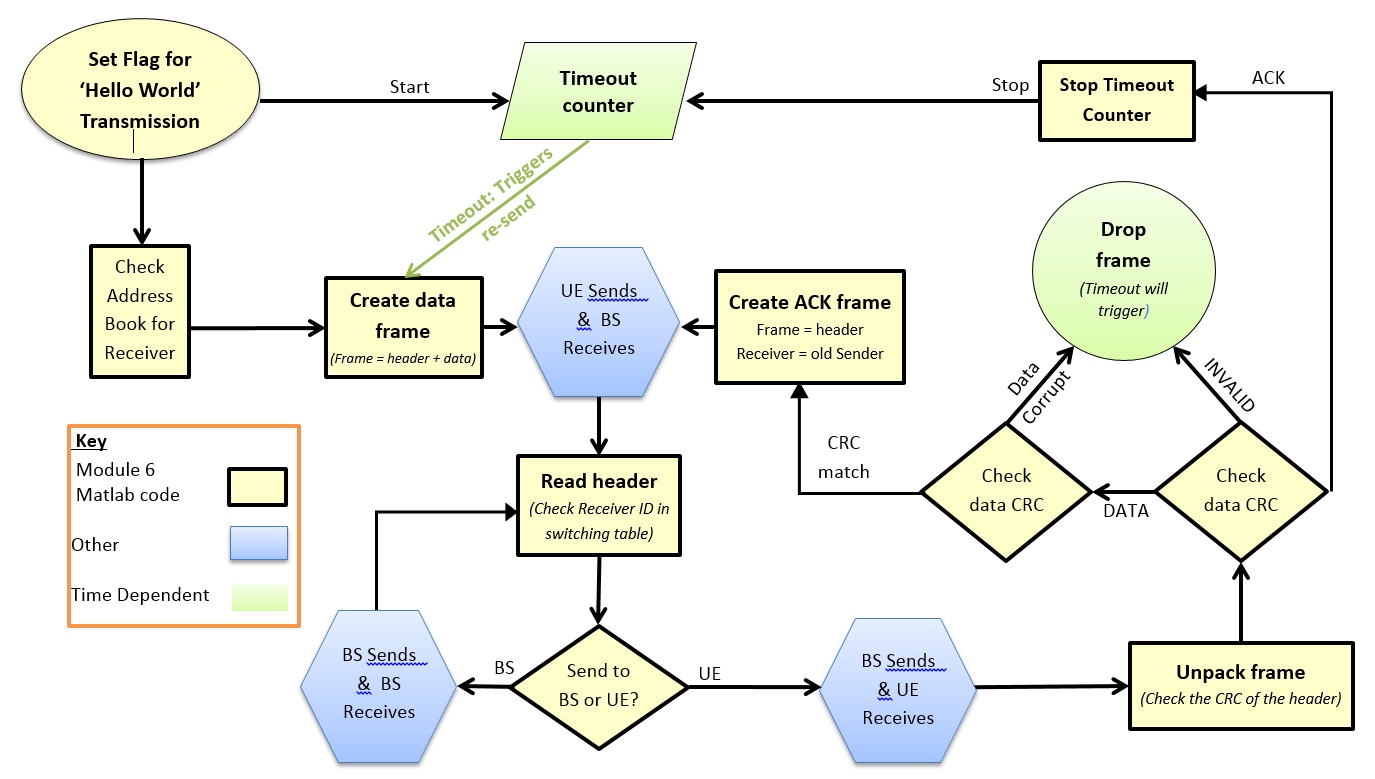
\includegraphics[width=0.8\textwidth]{Diagram.png}
    \caption{State Machine of transmission of package }
    \label{fig:stateMachine}
\end{figure}